%%── PANEL 3: Índice ─────────────────────────────────────────────────────────
\panel{LightBg}{%
  \vspace{3mm}
  {\small\bfseries\color{Navy}Contenido}
  \vspace{3pt}
  {\color{Navy!35}\rule{\linewidth}{0.5pt}}
  \vspace{2pt}

  \begin{enumerate}[leftmargin=14pt,itemsep=5pt,
                    label={\color{Navy}\bfseries\arabic*.}]
    \item {\scriptsize\textbf{Introducci\'on a la Teor\'ia de Ramsey}\\
      \tiny\color{gray!65}El principio del palomar y los n\'umeros de Ramsey.}

    \item {\scriptsize\textbf{El problema de la amistad}\\
      \tiny\color{gray!65}$K_6$ con 2-coloraci\'on siempre tiene tri\'angulo monocrom\'atico.}

    \item {\scriptsize\textbf{Coloraci\'on de enteros}\\
      \tiny\color{gray!65}$r$-coloraciones y conjuntos monocrom\'aticos.}

    \item {\scriptsize\textbf{Teorema de Schur (1916)}\\
      \tiny\color{gray!65}Toda coloraci\'on contiene $x+y=z$ monocrom\'atico.}

    \item {\scriptsize\textbf{Teorema de Van der Waerden (1927)}\\
      \tiny\color{gray!65}PA monocrom\'aticas de cualquier longitud.}

    \item {\scriptsize\textbf{Densidad natural}\\
      \tiny\color{gray!65}Conjuntos con $d(A)>0$ vs.\ $d(A)=0$.}

    \item {\scriptsize\textbf{Teorema de Szemer\'edi (1975)}\\
      \tiny\color{gray!65}$d(A)>0$ garantiza PA arbitrariamente largas.}

    \item {\scriptsize\textbf{Teorema de Green-Tao (2004)}\\
      \tiny\color{gray!65}Los primos ($d=0$) contienen PA de cualquier longitud.}

    \item {\scriptsize\textbf{Conclusiones}\\
      \tiny\color{gray!65}El orden es inevitable incluso en densidad cero.}
  \end{enumerate}

  \vfill
  {\color{Navy!30}\rule{\linewidth}{0.4pt}}
  \vspace{3pt}

  \begin{center}
  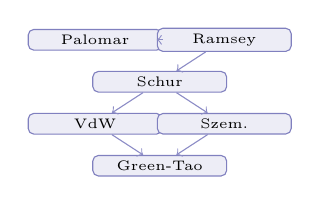
\begin{tikzpicture}[scale=0.82,
    nd/.style={draw=Navy!50,fill=Navy!7,rounded corners=2pt,
      font=\tiny,inner sep=2pt,minimum width=1.7cm,align=center}]
    \node[nd] (a) at (0,0)     {Palomar};
    \node[nd] (b) at (2.0,0)   {Ramsey};
    \node[nd] (c) at (1.0,-0.65){Schur};
    \node[nd] (d) at (0,-1.3)  {VdW};
    \node[nd] (e) at (2.0,-1.3){Szem.};
    \node[nd] (f) at (1.0,-1.95){Green-Tao};
    \foreach \s/\t in {a/b,b/c,c/d,c/e,d/f,e/f}
      \draw[->,Navy!45,thin] (\s)--(\t);
  \end{tikzpicture}
  \end{center}
}%
